\documentclass{article}
\author{}

\usepackage{graphicx}
\usepackage{wrapfig}
\usepackage{enumerate}
\usepackage{hyperref}
\usepackage{float}
\usepackage[margin = 2.25cm]{geometry}
\usepackage[table]{xcolor}
\usepackage{fancyhdr}
\hypersetup{
  colorlinks = true,
  urlcolor = blue
}
\setlength\parindent{0pt}
\pagestyle{fancy}
\fancyhf{}
\rhead{College of Engineering, Construction and Living Sciences\\Bachelor of Information Technology}
\lfoot{Practical 12 Django 6: Authentication \\Version 1, 2020}
\rfoot{\thepage}

\begin{document}

\begin{figure}
	\centering
	
\includegraphics[width=50mm]{./img/logo.png}
\end{figure}

\title{College of Engineering, Construction and Living Sciences\\Bachelor of Information Technology\\IN608: Intermediate Application Development Concepts\\Level 6, Credits 15\\\textbf{Practical 12 Django 6: Authentication}} 
\date{}
\maketitle

\textbf{Due Date:} 07/09/2020 at 5pm \\

In this practical, you will complete a series of tasks covering today's lecture. This practical is worth 1\% of the final mark for the IN608: Intermediate Application Development Concepts course. \\

Before you start, in your practicals repository, create a new branch called \textbf{12-practical}.

\section*{Task 1} 
Create a Django project called \texttt{quiz}. \texttt{cd} to \texttt{quiz}, create a virtual environment \& install Django. Create an app called \texttt{practical12quizcreator}. Please ensure you configure your app in \texttt{quiz/settings.py} \& \texttt{quiz/urls.py}. Install \texttt{Crispy Forms} Python module by running the command: \texttt{pipenv install django-crispy-forms}. Add \texttt{crispy\_form} to the \texttt{INSTALLED\_APPS} in \texttt{quiz/settings.py}. \\

In the \texttt{practical12quizcreator} directory, create a directory called \texttt{templates} \& two sub-directories called \texttt{practical12quizcreator} \& \texttt{registration}. In \texttt{templates/practical12quizcreator}, create three \texttt{HTML} files called \texttt{base.html}, \texttt{index.html} \& \texttt{details.html}. In \texttt{templates/registration}, create two \texttt{HTML} files called \texttt{login.html} \& \texttt{signup.html}. \\

In \texttt{models.py}, create two model classes called \texttt{User} which extends \texttt{AbstractUser} \& \texttt{Quiz} which extends \texttt{model.Model}. In \texttt{User}, declare the following field names with their types:
\begin{verbatim}
  username = models.CharField(max_length=25, unique=True, blank=False)
  email = models.EmailField(unique=True, blank=False)
  first_name = models.CharField(max_length=200, blank=False)
  last_name = models.CharField(max_length=200, blank=False)
\end{verbatim}

For \texttt{User}, create a \texttt{\_\_str\_\_} method which returns \texttt{first\_name} \& \texttt{last\_name}. \\

In \texttt{Quiz}, declare the following choices:
\begin{verbatim}
  CATEGORIES = [(' ', 'Any Category'),
                ('9', 'General Knowledge'),
                ('18', 'Science: Computers'),
                ('21', 'Sport'),
                ('22', 'Geography'),
                ('27', 'Animals')]
  DIFFICULTIES = [(' ', 'Any Difficulty'),
                  ('easy', 'Easy'),
                  ('medium', 'Medium'),
                  ('hard', 'Hard')]
\end{verbatim}

If you want to add more categories, view the following API: \href{https://opentdb.com/api\_category.php}{https://opentdb.com/api\_category.php}. \\

Below the two choices, declare the following field names with their types:

\begin{verbatim}
  creator = models.ForeignKey(User, on_delete=models.CASCADE)
  name = models.CharField(max_length=200, null=False)
  category = models.CharField(max_length=200, choices=CATEGORIES, null=False)
  difficulty = models.CharField(max_length=200, choices=DIFFICULTIES, null=False)
\end{verbatim}

For \texttt{User}, create a \texttt{\_\_str\_\_} method which returns \texttt{name} \\

Create a file called \texttt{forms.py}, create two form classes called \texttt{SignupForm} which extends \texttt{auth\_forms.UserCreationForm} \& \texttt{QuizForm} which extends \texttt{forms.ModelForm}. \textbf{Note:} please ensure you declare the following:

\begin{verbatim}
  from django import forms
  from django.contrib.auth import forms as auth_forms
  from .models import Quiz, User
\end{verbatim}

\texttt{SignupForm} contains the model \texttt{User} \& the fields \texttt{username}, \texttt{first\_name}, \texttt{last\_name} \& \texttt{email}. \texttt{QuizForm} contains the model \texttt{Quiz} \& the fields \texttt{name}, \texttt{category} \& \texttt{difficulty}. \\

In \texttt{views.py}, create three classes called \texttt{SignupView} which extends \texttt{generic.FormView}, \texttt{IndexView} which extends \texttt{generic.FormView} \& \texttt{DetailsView} which extends \texttt{generic.ListView}. \texttt{SignupView} has a method called \texttt{form\_valid} which creates a \texttt{User}, logs the \texttt{User} in \& redirects to \texttt{index.html}. \texttt{IndexView} has a method called \texttt{form\_valid} which creates a \texttt{Quiz} \& redirects to \texttt{index.html}. \texttt{DetailsView} has a method called \texttt{get\_queryset} which returns a \texttt{QuerySet} containing all \texttt{Quiz} objects. \\

Create a file called \texttt{urls.py} in the \texttt{practical12quizcreator} app directory. In \texttt{urls.py}, set the \texttt{app\_name} to \texttt{practical09dogsearch} \& create three URLs which map to the \texttt{SignupView} class, \texttt{IndexView} class \& \texttt{DetailsView} class in \texttt{views.py}. Create two more URLs for \texttt{LoginView} \& \texttt{LogoutView} auth views.

\subsection*{Expected Output} 
Run the command \texttt{python manage.py runserver} then navigate to \href{http://127.0.0.1:8000/practical12quizcreator/}{http://127.0.0.1:8000/practical12quizcreator/} \\ 

\texttt{login.html} - login using a valid username \& password (both fields are required). If successful, the user is redirected to \texttt{index.html}. If a user wants to signup, they can click the \texttt{here} link which will redirect the user to \texttt{signup.html}.

\begin{figure}[H]
  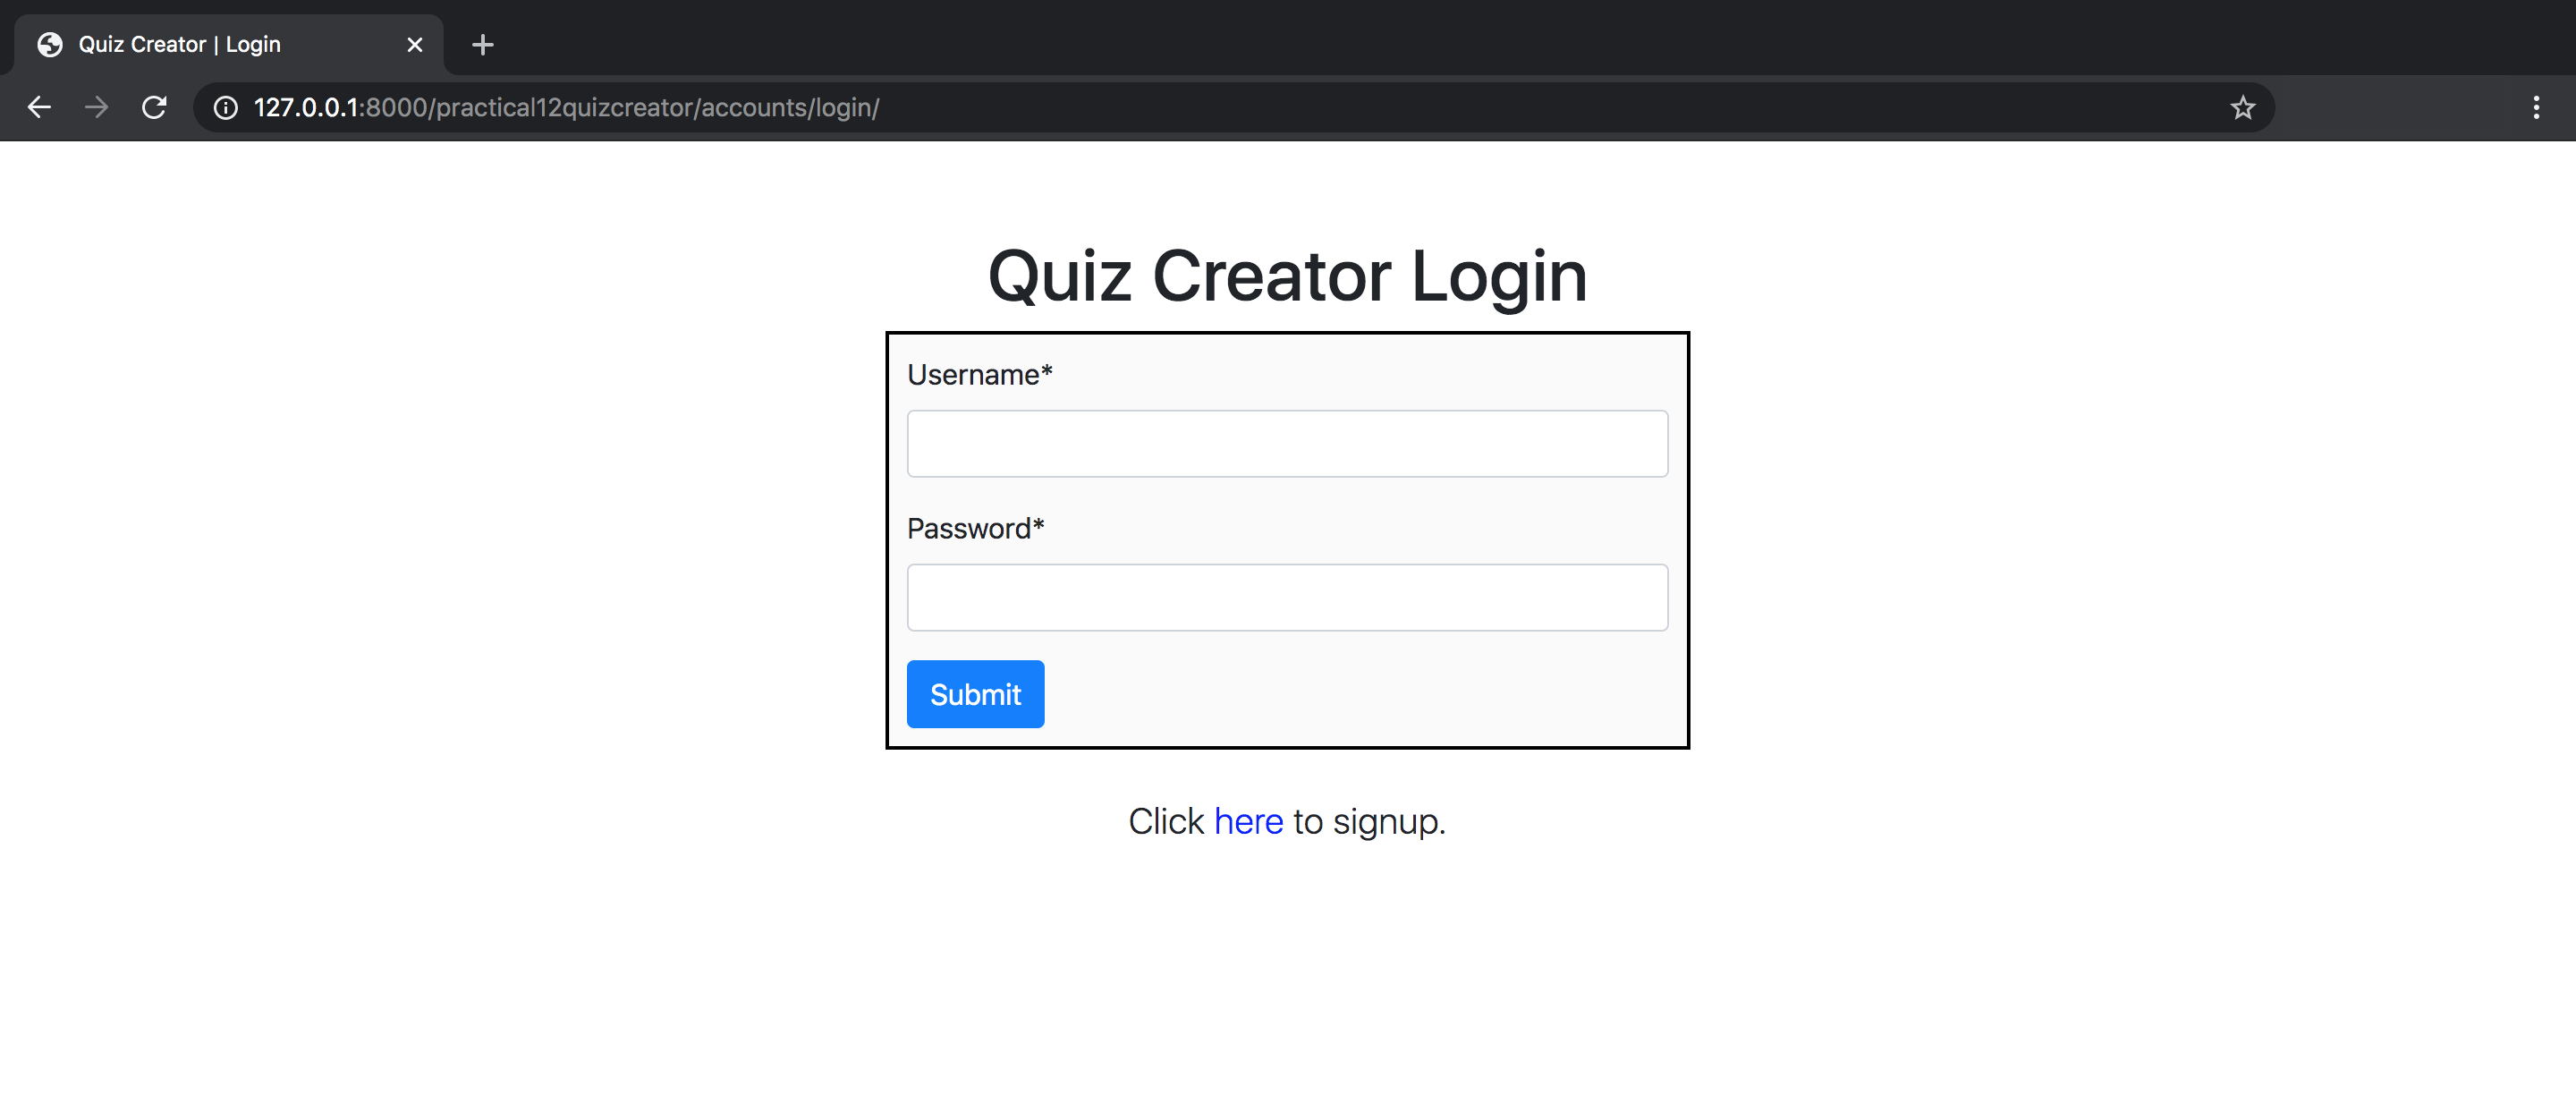
\includegraphics[width=175mm, height=75mm]{./img/12-expected-quiz-1.png}
\end{figure}

\texttt{signup.html} - all fields are required. If an email already exists, then the user must enter a different email. Password has additional validation:
\begin{itemize}
  \item Can not be too similar to your other personal information
  \item Must contain at least 8 characters
  \item Can not be a commonly used password
  \item Can not be entirely numeric
\end{itemize}

If successful, the user is redirected to  \texttt{index.html}. 

\begin{figure}[H]
  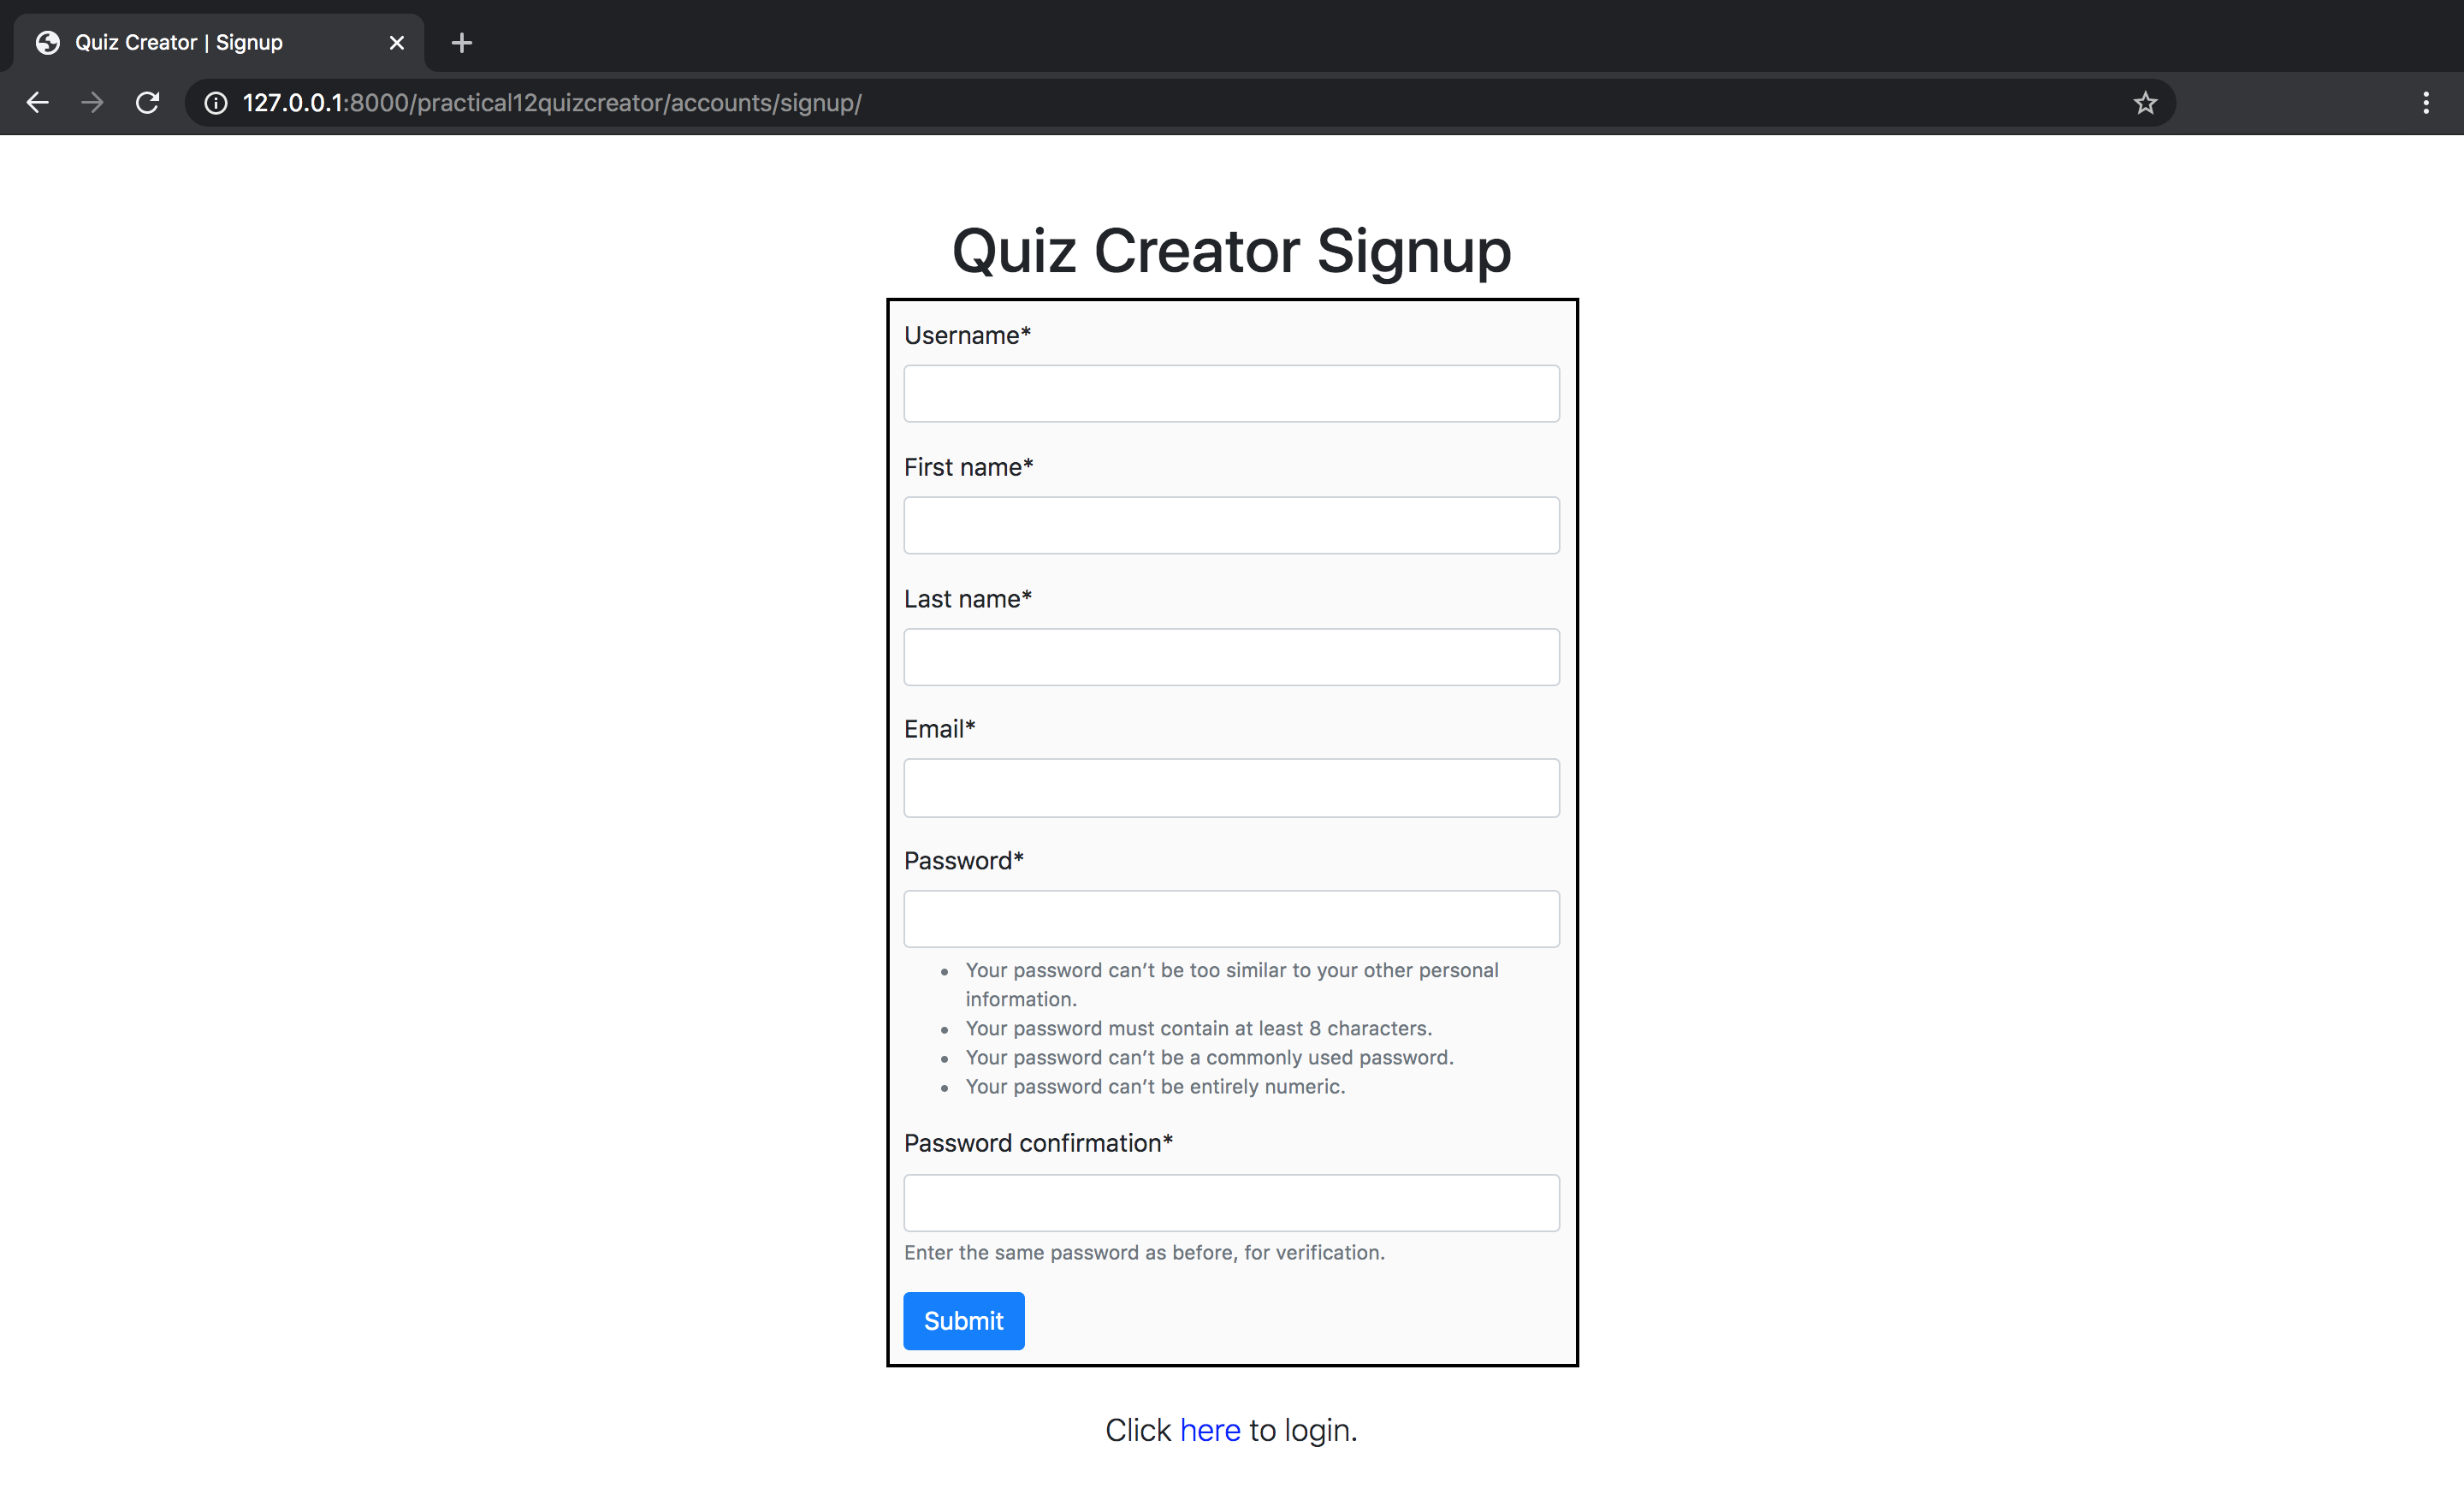
\includegraphics[width=175mm, height=100mm]{./img/12-expected-quiz-2.png}   
\end{figure}

\newpage

\texttt{index.html} - all fields are required. If a user navigates to \texttt{index.html} \& is not authenticated, the user is redirected to \texttt{login.html}. Select drop downs are populate via choices in \texttt{models.py}. If the form is valid, a \texttt{Quiz} is created. If a user wants to logout, they can click the \texttt{Logout} link which will redirect the user to \texttt{login.html}.

\begin{figure}[H]
  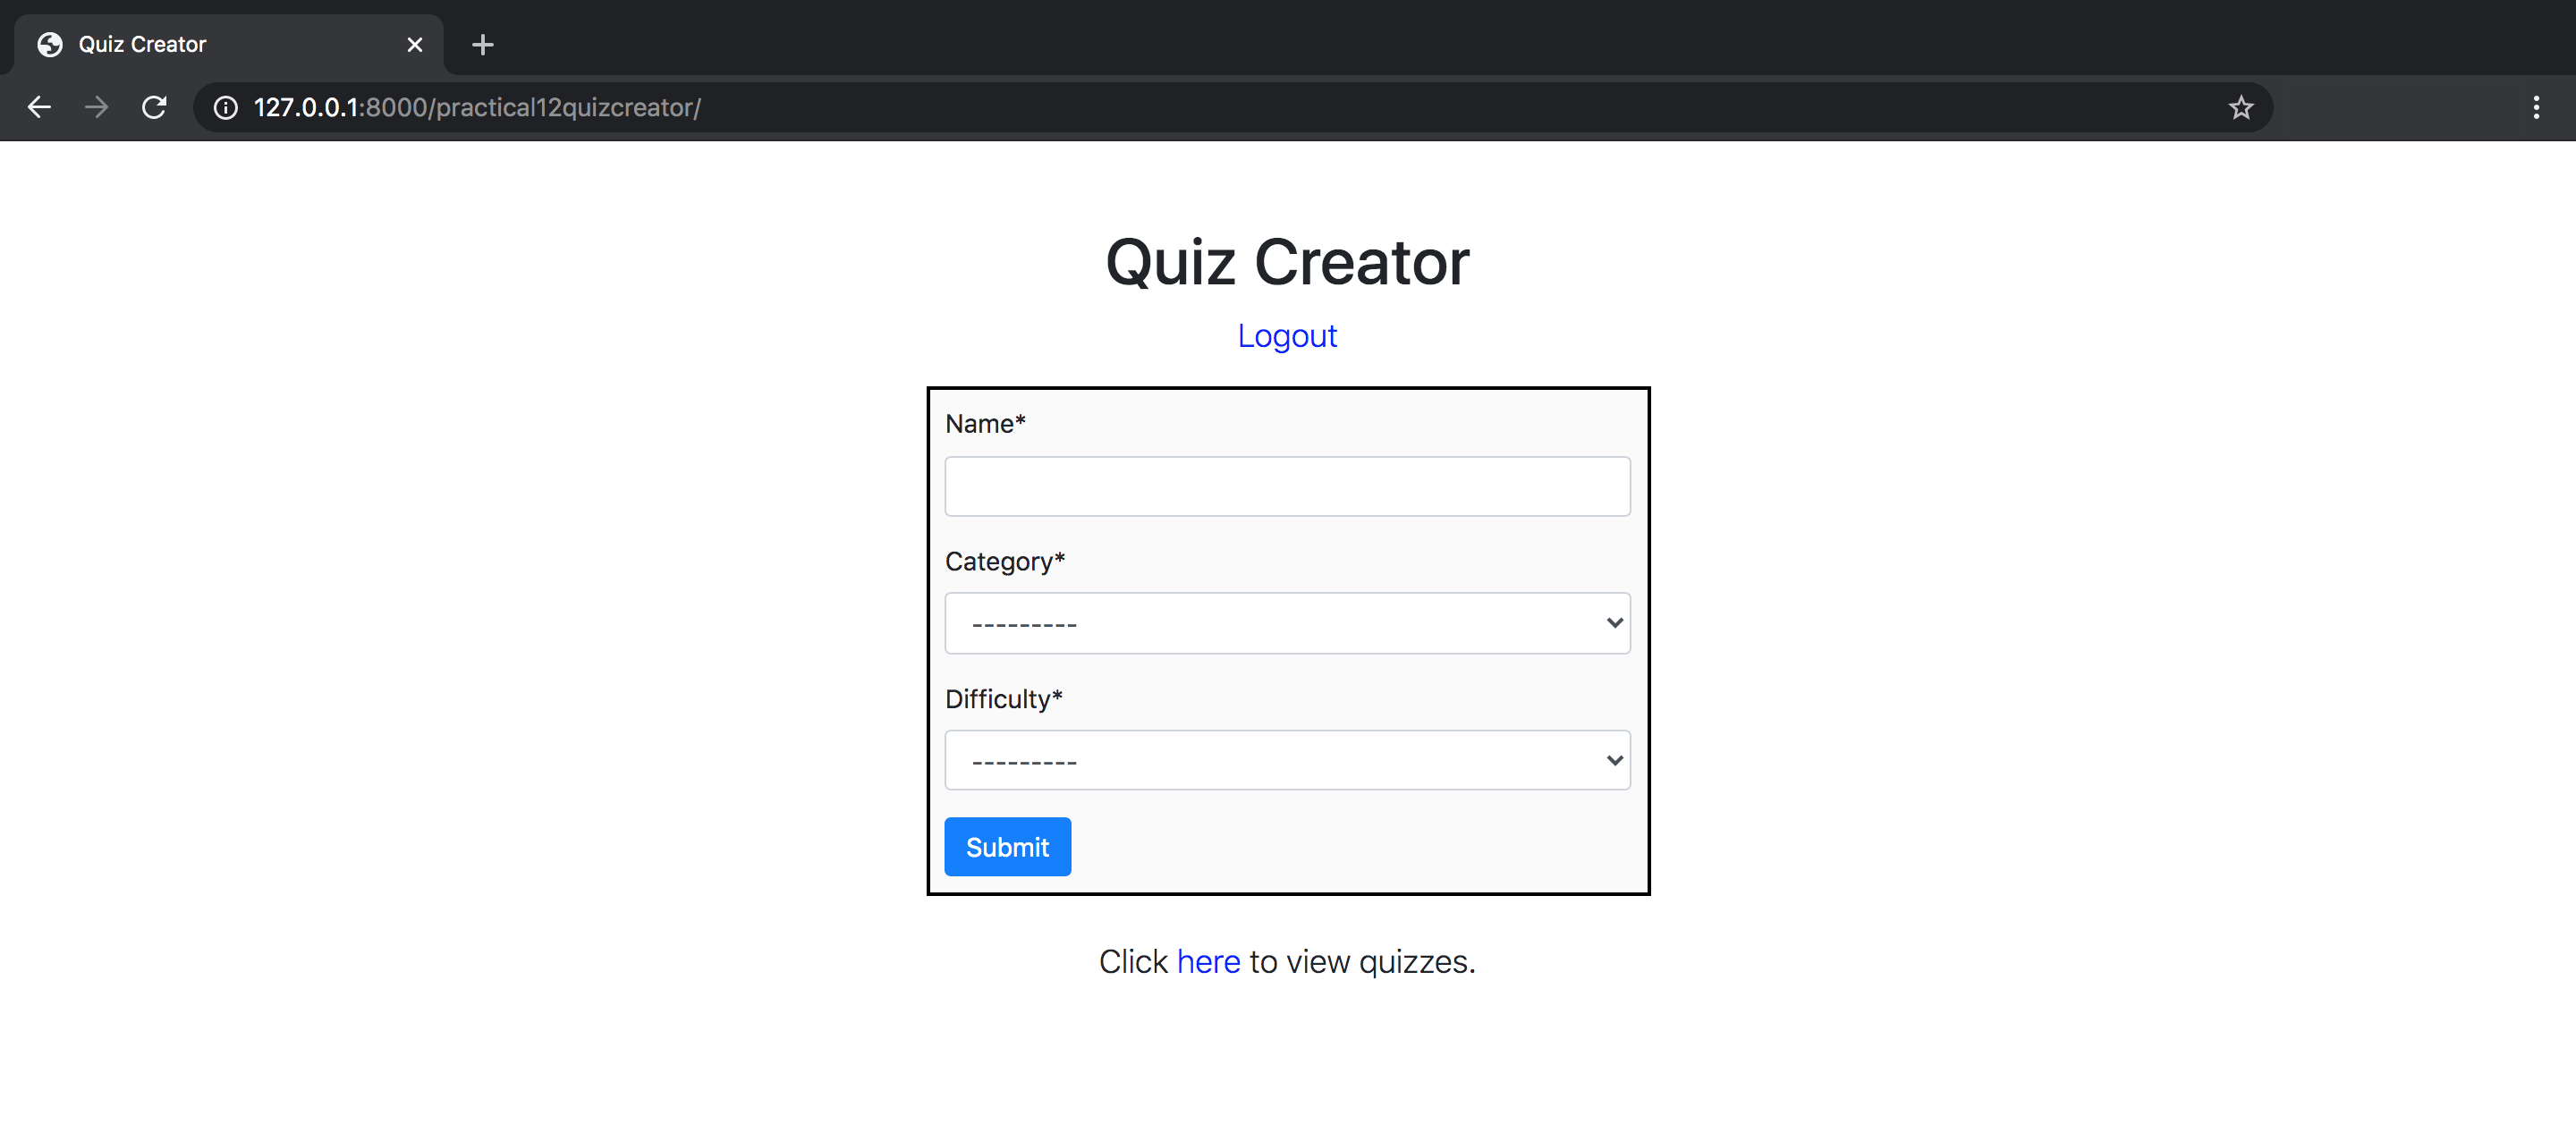
\includegraphics[width=175mm, height=75mm]{./img/12-expected-quiz-3.png}
\end{figure}

\begin{figure}[H]
  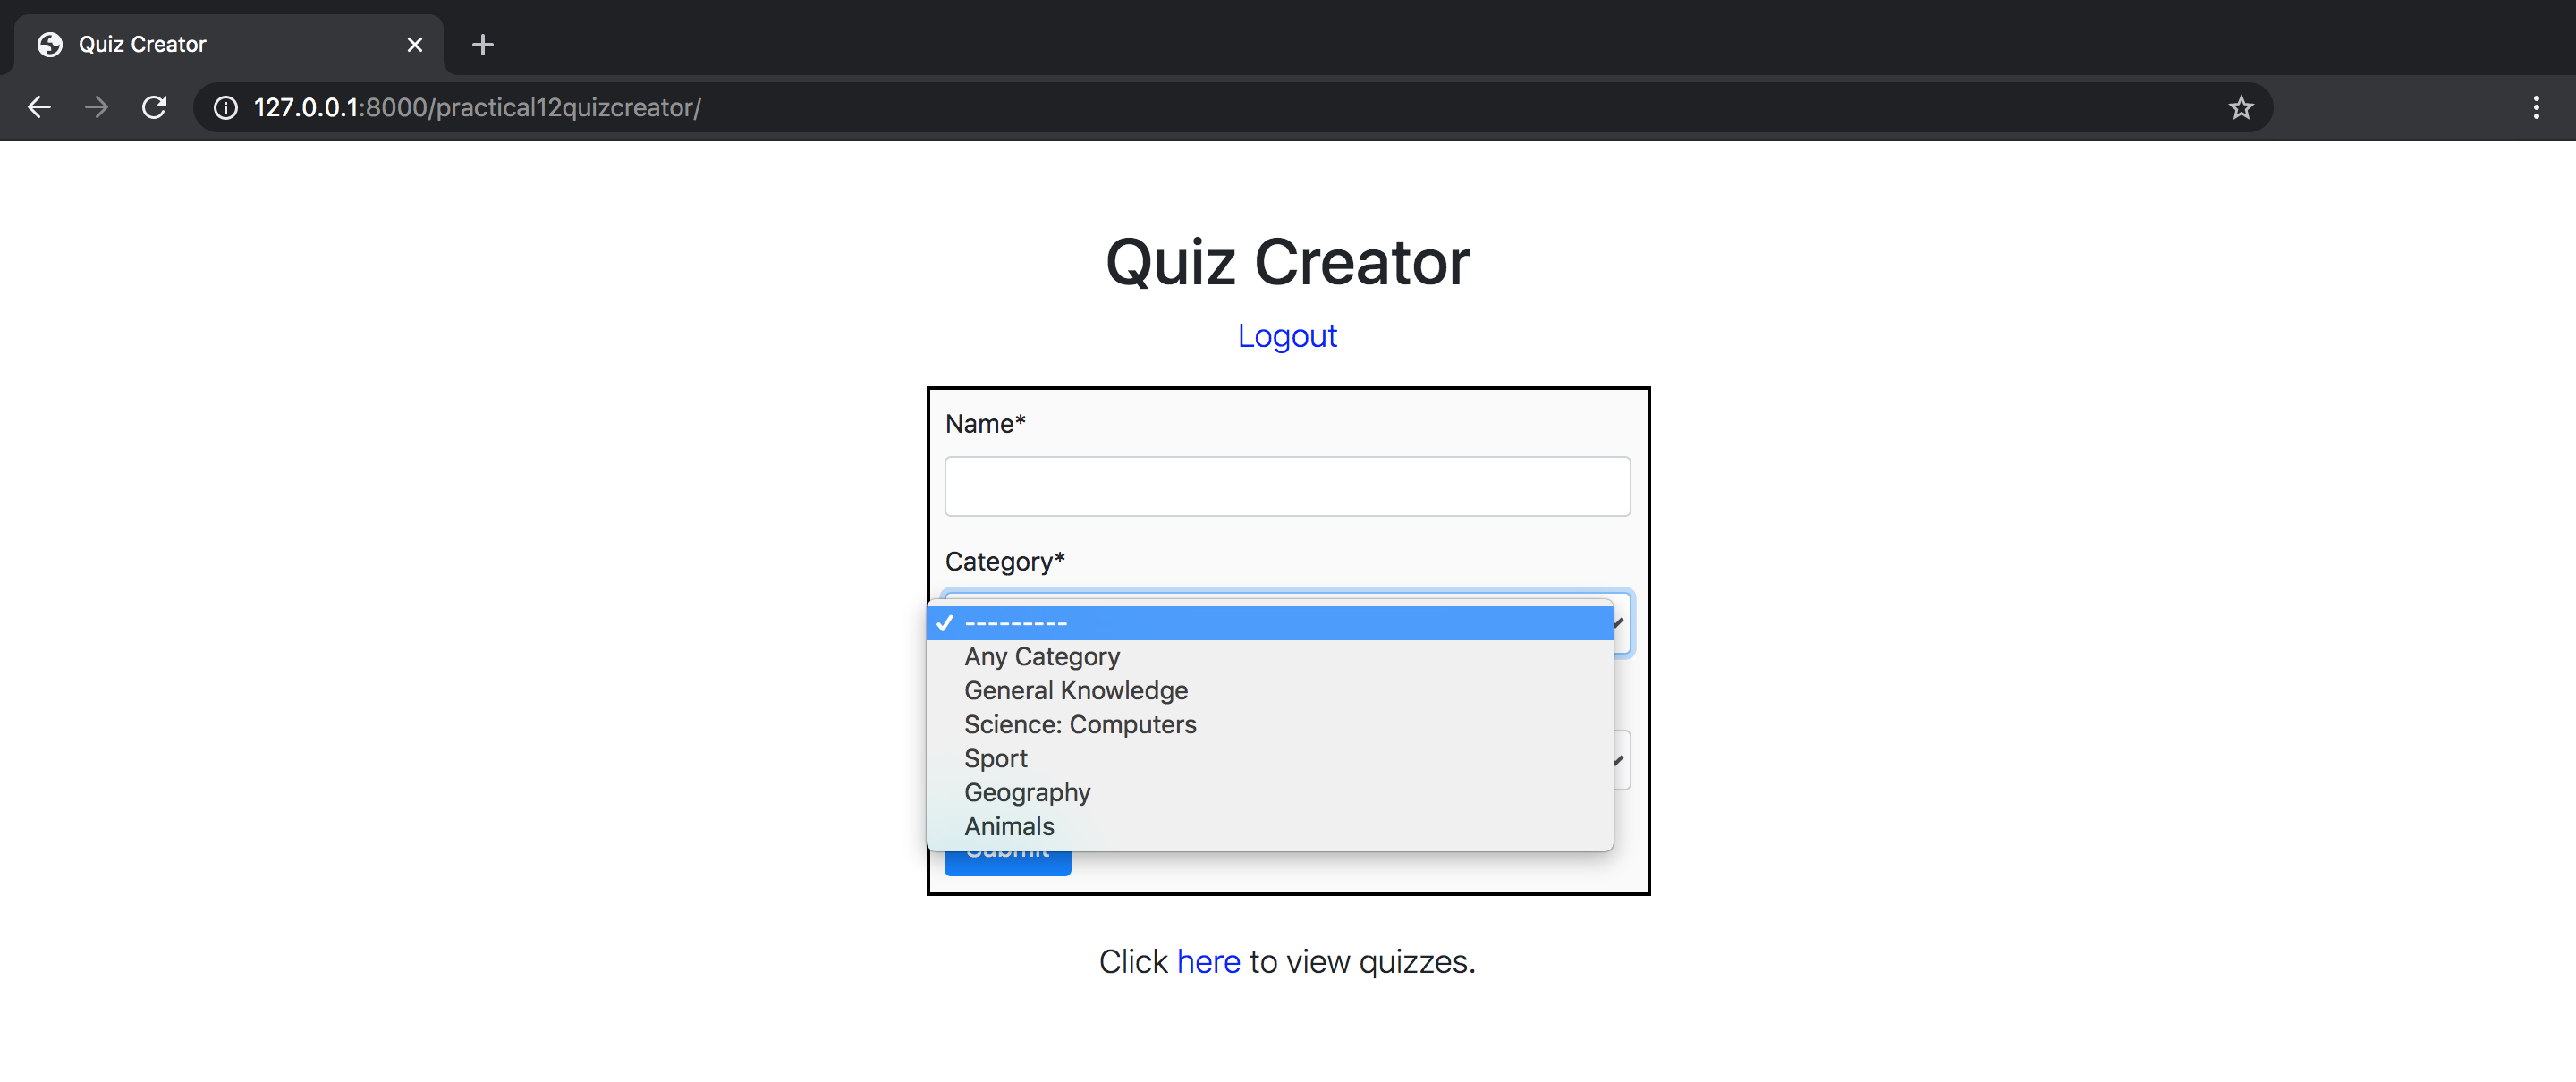
\includegraphics[width=175mm, height=75mm]{./img/12-expected-quiz-4.png}
\end{figure}

\begin{figure}[H]
  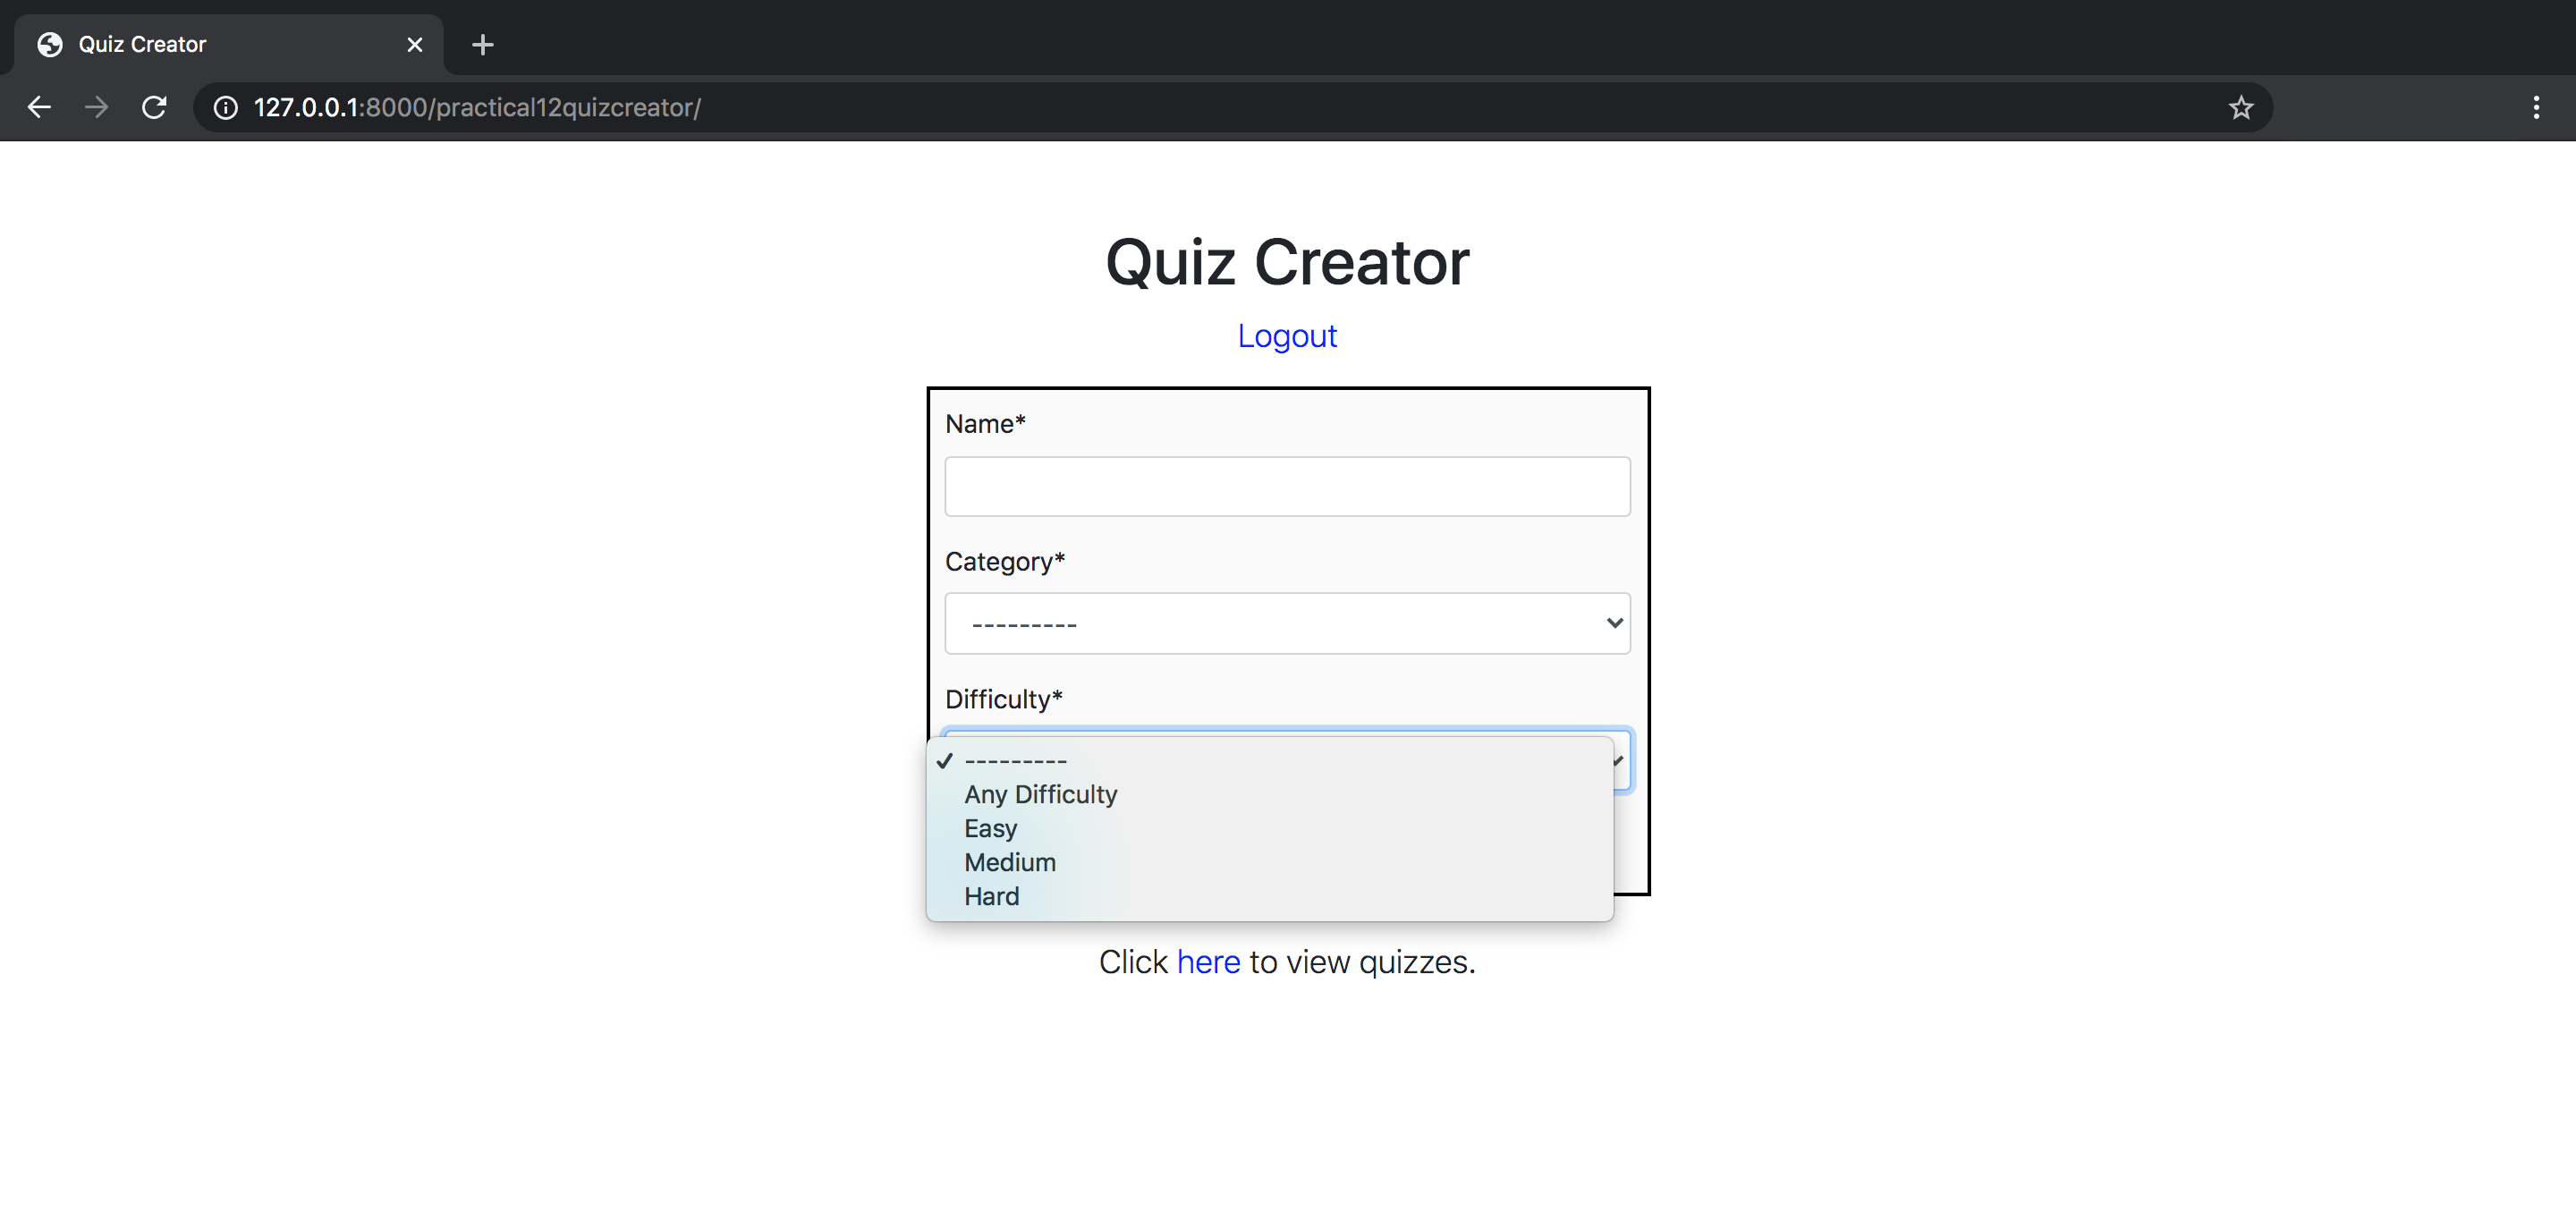
\includegraphics[width=175mm, height=75mm]{./img/12-expected-quiz-5.png}
\end{figure}


\begin{figure}[H]
  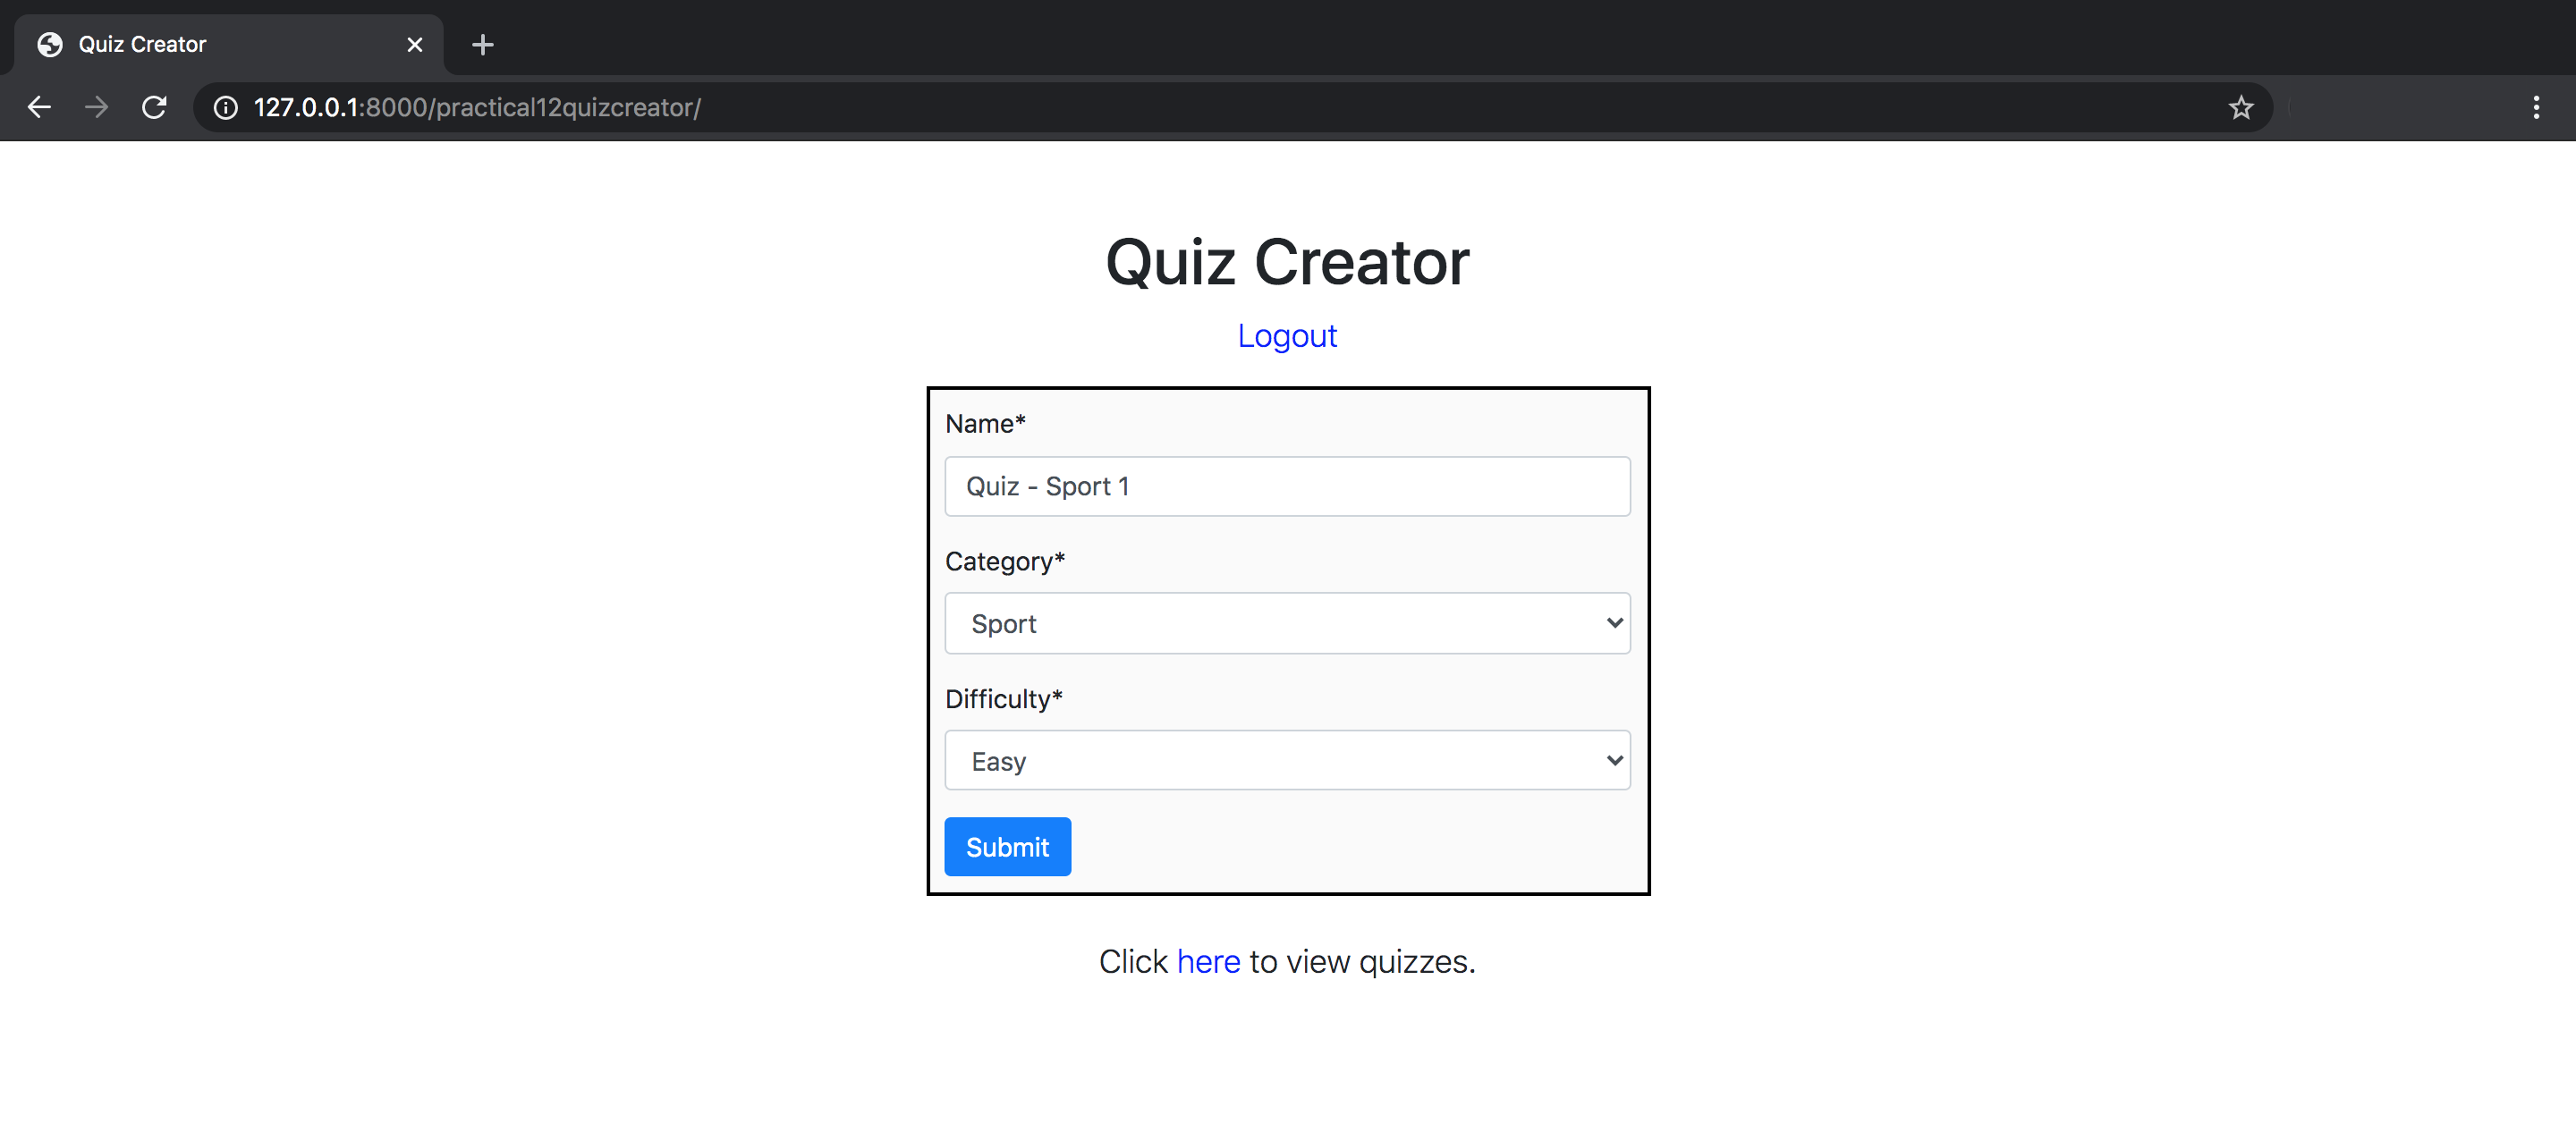
\includegraphics[width=175mm, height=75mm]{./img/12-expected-quiz-6.png}
\end{figure}

\texttt{details.html} - display all \texttt{Quiz} objects in a nicely formatted HTML table.

\begin{figure}[H]
  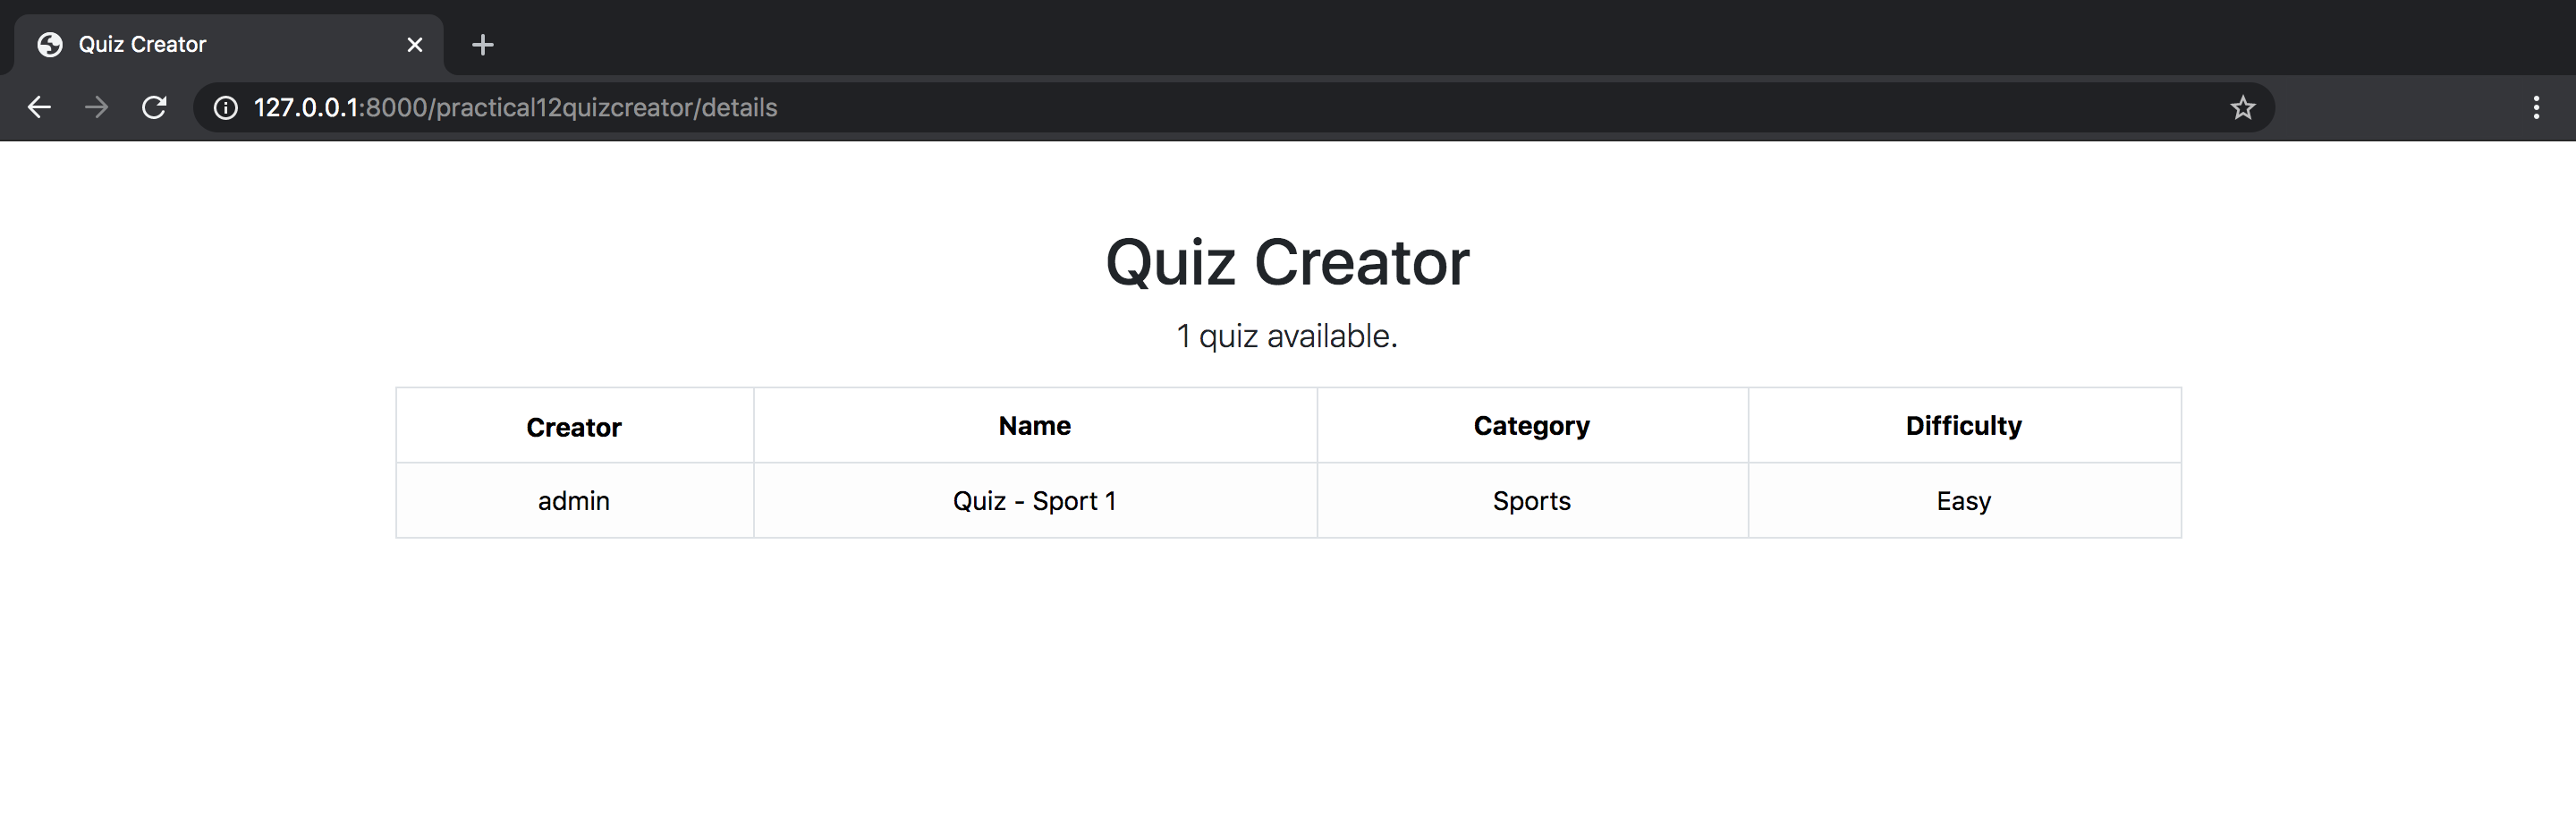
\includegraphics[width=175mm, height=55mm]{./img/12-expected-quiz-7.png}
\end{figure}

\textbf{Deployment link:} \href{https://int-app-dev-practical-12.herokuapp.com/practical12quizcreator/}{https://int-app-dev-practical-12.herokuapp.com/practical12quizcreator/}

\section*{Task 2} 
Write the following unit tests:
\begin{itemize}
  \item Signup is successful \& unsuccessful
  \item Login is successful \& unsuccessful
  \item Quiz is successfully created 
\end{itemize}

Write the following end-to-end test:
\begin{itemize}
  \item Login, create a quiz \& view all quizzes
\end{itemize}

\end{document}